% Manuscript prepared for Electronics (MDPI), Artificial Intelligence section.
% Special Issue: Trustworthy AI for Large Models and Security Systems.
% Compile inside the official MDPI LaTeX template.
% Before submission, verify the journal option against the current MDPI template
% and complete all author declarations in the submission system.
\documentclass[electronics,article,submit,pdftex,moreauthors]{Definitions/mdpi}

\Title{Information Leakage from Token-Length Traces in Streaming LLMs: Cross-Model Reconstruction and Defense Evaluation}
\Author{Paweł Augustynowicz $^{1,*}$ and Szymon Jędrzejczak $^{1,*}$}
\AuthorNames{Paweł Augustynowicz and Szymon Jędrzejczak}
\address[1]{Faculty of Cybernetics, Military University of Technology, gen. Sylwestra Kaliskiego 2, 00-908 Warsaw, Poland; pawel.augustynowicz@wat.edu.pl (P.A.); szymon.jedrzejczak@wat.edu.pl (S.J.)}
\corres{Correspondence: pawel.augustynowicz@wat.edu.pl (P.A.); szymon.jedrzejczak@wat.edu.pl (S.J.)}

\pubvolume{1}
\issuenum{1}
\articlenumber{0}
\pubyear{2026}
\copyrightyear{2026}
\datereceived{}
\daterevised{}
\dateaccepted{}
\datepublished{}

\usepackage{booktabs}
\usepackage{multirow}
\usepackage{graphicx}
\usepackage{array}
\usepackage{longtable}
\usepackage{tabularx}
\usepackage{threeparttable}
\usepackage{amsmath}
\usepackage{enumitem}
\usepackage{placeins}
\usepackage{tikz}
\usetikzlibrary{arrows.meta,positioning,shapes.geometric,fit}
\setlength{\headheight}{24pt}

\abstract{Streaming large language model (LLM) services can expose response-length metadata even when payloads are encrypted. We evaluate a fixed T5 reconstructor through 6600 reconstructions from validated application-layer length traces. For 300 aligned prompts per model, five archived-reference cohorts yield mean term-frequency cosine scores ($\phi$) of 0.482--0.535; two additional archived cohorts have malformed word boundaries. Newly generated TinyLlama and Phi-3.5-mini responses with verified detokenization yield means of 0.435 and 0.504. Legacy rendering of their saved token IDs reproduces all 600 corresponding archived references and length vectors. Changing both the trace and scoring reference increases mean $\phi$ by 0.356 and 0.383 under matched reconstruction settings. In two-model pilots, three of six partial-ablation contrasts remain significant after Holm correction; neither cross-prompt contrast is conclusive. Five framing transformations reduce frozen-reconstructor mean scores by 36.7--88.7\%. A five-seed study with a maximum-a-posteriori (MAP) length inverse recovers much of the loss under bucketing and batching. Reconstruction scopes and retained encoder coverage differ across these experiments. The findings quantify lexical behavior of an instrumented pipeline and demonstrate the importance of validating both observations and reference rendering. They do not measure semantic disclosure or demonstrate passive extraction from encrypted transport.}

\keyword{large language models; information leakage; side-channel analysis; server-sent events; traffic analysis; token-length traces; text reconstruction; privacy}

\begin{document}

\section{Introduction}
Interactive large language model (LLM) services stream partial responses to reduce latency. One implementation uses Server-Sent Events (SSE), with generated text carried in application events. Encryption hides the event contents but not necessarily the shape of the communication. If application-event boundaries or correlated record sizes are observable, a sequence of lengths can reveal properties of the underlying tokens.

This paper separates reconstruction from a known length trace from extraction of that trace from encrypted traffic. The laboratory observable is the ordered UTF-8 byte length of each token fragment emitted by an instrumented service, before transport processing. A validated log oracle supplies these lengths and preserves newline bytes and empty fragments. This abstraction removes segmentation by HTTP and Transport Layer Security (TLS), buffering, retransmission, and multiplexing from the experiment. The historical line-collector discrepancy motivates the validation in Section~\ref{sec:measurement-audit}; all quantitative reconstruction results reported below use recorded, validated input vectors. No experiment here establishes passive extraction of event boundaries from encrypted traffic.

Building on Weiss \emph{et al.}, who reconstructed streamed responses from token-length patterns using a T5-based inversion pipeline~\cite{weiss2024prompt}, we examine one fixed reconstructor across open-weight victim models. Partial trace ablations assess its sensitivity to ordered lengths, and framing transformations test its response without retraining. The seven-model cohort retains archived emitted texts; TinyLlama and Phi-3.5-mini are diagnostic within that cohort because of malformed word boundaries. A separate two-model experiment uses newly generated responses with verified full-sequence detokenization.

The study addresses three research questions:
\begin{enumerate}[label=\textbf{RQ\arabic*:},leftmargin=4.2em,labelwidth=3.2em,labelsep=0.6em]
    \item Do ordered logged lengths improve lexical scores over controls that shuffle lengths, replace them with a constant, or use another prompt's trace?
    \item How do scores from validated length traces differ across seven archived victim-model cohorts, and how do separate experiments with verified reference decoding inform the two diagnostic series?
    \item How do bucketing, fixed-width units, batching, and randomized padding affect the evaluated pipeline, protected-payload size, and observable-unit count, and how does a prompt-disjoint maximum-a-posteriori (MAP) inverse change its scores?
\end{enumerate}

The contribution is an evaluation with explicit input provenance: 2100 reconstructions from validated archived lengths, 600 additional reconstructions of newly generated and correctly assembled responses, two-model pilots of partial trace ablations and five framing configurations, and a five-seed MAP-inverse evaluation. The pilots and MAP study use different reconstruction scopes, so their baselines are not interchangeable. Full input vectors, decoder inputs, random seeds, generated texts, and independent metric checks are retained in the accompanying artifact package. The source project is hosted at \url{https://github.com/jackaugustyn/LLeakM}. Appendix~\ref{app:runs} identifies the completed experiment artifacts and distinguishes them from historical manifests.

\section{Related Work}
Side-channel attacks infer sensitive information from indirect observables such as timing and message size. Classical timing attacks showed that implementation-level leakage can defeat cryptographic protection without recovering plaintext directly~\cite{kocher1996timing}. Encrypted network applications likewise leak through packet sizes and timing. Keystroke inference, web-application traffic analysis, and website fingerprinting demonstrate that encryption does not hide communication shape~\cite{song2001timing,chen2010sidechannel,cai2012touching,sirinam2018deep}.

Traffic-analysis defenses transform that shape through padding, morphing, batching, or cover traffic. Traffic morphing attempts to make one traffic class resemble another, while subsequent studies show that efficient countermeasures may retain exploitable structure or impose substantial overhead~\cite{wright2009morphing,dyer2012peekaboo}. For this reason, defense effectiveness should be evaluated by reporting both the leakage that remains and the resulting bandwidth and latency overhead, rather than by treating padding as either fully protective or ineffective.

For generative AI, Weiss \emph{et al.} introduced T5-based sequence-to-text inversion and reported accurate reconstruction for 27\% of responses and topic inference for 53\% in their evaluated setting~\cite{weiss2024prompt}. Li \emph{et al.} subsequently studied API outputs that merge several tokens into one observable unit and showed that aggregation does not remove the side channel~\cite{li2026length}. Whisper Leak instead infers prompt topics from packet-size and timing patterns in encrypted LLM traffic~\cite{whisperleak2025}. Those studies address stronger deployment-facing threat models. The present work narrows the observation layer to ask a different question: how a fixed reconstructor transfers across victim models once a token-granular length trace is available, and how simple transformations affect that same reconstructor.

The reconstruction pipeline uses T5-style text-to-text transformers~\cite{raffel2020exploring}. Evaluation combines a reference-normalized Levenshtein distance~\cite{levenshtein1966binary}, ROUGE precision~\cite{lin2004rouge}, and one fixed term-frequency cosine score $\phi$. These are lexical measures. They should not be read as semantic correctness or disclosure of a usable answer.

\section{Materials and Methods}
\subsection{Threat Model and Objective}
We evaluate a length-only reconstructor for an instrumented LLM service. The observation is the ordered byte length of each emitted token fragment; the attacker receives neither the generating prompt, token identities, nor victim-model internals. The evaluator uses instrumented logs to verify these lengths and to obtain reference text, but supplies only the lengths to the reconstructor. This application-layer oracle does not recover event boundaries from TLS, HTTP/2, or QUIC traffic. The archived-reference cohort and the newly generated two-model cohort are kept separate because verified byte lengths do not themselves establish ordinary detokenization of historical outputs.

The objective is to characterize lexical reconstruction in this controlled apparatus and the response of a fixed reconstructor to length transformations. The experiments capture per-token traces, reconstruct text from length sequences, and compare the reconstructions with the stored emitted responses. Prompts are used to generate those responses and are not supplied to the reconstructor. Figure~\ref{fig:threat_model} shows the intended information flow.

\subsection{Information-Theoretic Interpretation}
Let $R$ denote the stored emitted response and let $X=(L_1,\ldots,L_T)$ denote its ordered token-payload length trace in the idealized laboratory model. When a defense is applied, $X$ is transformed into the observable trace $Z=g(X,N)$, where $N$ is independent transformation randomness. The attacker produces $\widehat{R}=A(Z,U)$ using independent decoder randomness $U$. Conditional on a fixed fitted attacker, these relationships form the following Markov chain:
\begin{equation}
R \longrightarrow X \longrightarrow Z \longrightarrow \widehat{R}.
\end{equation}
According to the data-processing inequality,
\begin{equation}
I(R;\widehat{R}) \leq I(R;Z) \leq I(R;X).
\end{equation}
Neither processing stage increases mutual information about $R$ under these assumptions. The empirical controls are partial trace ablations: they preserve response-dependent features such as trace length, the length histogram, or mean length. A score advantage over an ablation indicates sensitivity to the altered features, but does not isolate all trace information from the decoder's language prior. The lexical score $\phi$ does not estimate mutual information, and its reduction for a fixed attacker does not measure defended-channel capacity.

\begin{figure*}[ht]
\centering
\resizebox{0.96\textwidth}{!}{%
\begin{tikzpicture}[>=Latex,font=\small,
box/.style={draw,rounded corners,align=center,minimum height=12mm,text width=32mm,fill=blue!5},
obs/.style={box,fill=orange!12},eval/.style={box,fill=gray!10}]
\node[box] (prompt) at (0,0) {Synthetic prompt corpus};
\node[box] (victim) at (4.1,0) {Local victim model\\text generation};
\node[box] (records) at (8.2,0) {Logged text fragments\\and payload bytes};
\node[obs] (lengths) at (4.1,-1.8) {Validated trace $X$\\ordered byte lengths\\(UTF-8)};
\node[eval] (reference) at (8.2,-1.8) {Emitted reference $R$\\evaluator only};
\node[box,fill=green!6] (attacker) at (4.1,-3.6) {Fixed T5 reconstructor\\length input only};
\node[eval] (metrics) at (8.2,-3.6) {Lexical evaluation\\compare $\widehat R$ with $R$};
\draw[->] (prompt)--(victim);
\draw[->] (victim)--(records);
\draw[->] (records.south west)--(lengths.north east);
\draw[->] (records)--(reference);
\draw[->] (lengths)--(attacker);
\draw[->] (reference)--(metrics);
\draw[->] (attacker)--node[above] {$\widehat R$} (metrics);
\node[align=left,text width=31mm,font=\footnotesize] at (0,-2.6)
{The attacker receives neither the prompt nor reference text.\\[3pt]
Transport extraction and timing are outside this experiment.};
\end{tikzpicture}%
}
\caption{Information flow in the instrumented experiment. Logged fragments supply two separate evaluator products: a validated length trace and the emitted reference text. Only the lengths enter the reconstructor; the reference is used for scoring. The diagram makes no assumption that an instrumented write is a valid SSE event or an observable encrypted-transport record.}
\label{fig:threat_model}
\end{figure*}

\subsection{Streaming Harness and Trace Collection}
The instrumented harness associates each generated token position with a text fragment and records its UTF-8 length, serialized-write length, and relative timestamp. The historical implementation decoded each token independently; the new-generation implementation uses contextual prefix decoding and verifies that the fragments concatenate exactly to the full decoded token sequence. The new harness completes token generation and contextual decoding before emitting the fragments; it validates payload lengths rather than the timing of incremental generation. Each write has the SSE-like serialization \texttt{data: \textless fragment\textgreater\textbackslash n\textbackslash n}, and termination uses \texttt{data: [DONE]\textbackslash n\textbackslash n}. Raw newlines inside fragment text are not escaped, so a write is not necessarily a valid single SSE data event. The present experiments use validated lengths from the instrumented logs, not a line-based parser.

For the logged serialization, the payload length satisfies
\begin{equation}
L^{\mathrm{log}}_t = L^{\mathrm{write}}_t - 8,
\end{equation}
where the eight bytes are the prefix \texttt{data: } and suffix \texttt{\textbackslash n\textbackslash n}. This identity concerns the complete emitted byte string, including newline bytes inside the fragment. The terminal \texttt{[DONE]} write is excluded. Validation checks per-fragment byte counts, their order, concatenated reference text, total payload bytes, and sample/log identity. For newly collected streams the collector also checks the total received byte count. Exact vectors, source hashes, and reference text are saved with every reconstruction input. The primary, control, defense, and MAP experiments all use this explicit log-length representation.

\subsection{Measurement and Reference-Text Audit}\label{sec:measurement-audit}
The archived collector used \texttt{requests.iter\_lines()}, discarded empty lines, and appended two newline bytes to each remaining line. Its inferred vector $X^{\mathrm{col}}$ can differ from the logged vector $X^{\mathrm{log}}$: a fragment \texttt{:\textbackslash n\textbackslash n} contains three bytes, but this parser infers one. Replaying that implementation on the retained logs changes 2073 of 2100 vectors and the heuristic-segment count in 764 samples. These are preprocessing comparisons; the exact historical T5 input vectors and their binding to the old collector version were not retained.

The primary results below instead come from complete T5 inference on the 2100 validated logged vectors. This establishes the inputs used for the reported reconstructions without recovering undocumented historical inputs. Differences from older scores cannot be attributed solely to collection: the execution environment and reconstruction random-state handling also differ. The reconstructor is seeded after checkpoint loading so that cache initialization does not change a sample's random stream.

Reference text requires a separate check. The historical harness's independent token decoding produced no ASCII spaces in 299/300 TinyLlama responses and 162/300 Phi-3.5-mini responses. Those 600 archived references remain diagnostic; validating their emitted byte lengths does not restore their word boundaries. Historical token IDs are unavailable for all seven models, so complete-sequence detokenization of the other archived series is also not certified.

To evaluate the affected models with ordinary reference text, we generated 300 additional responses per model from the same prompts using contextual detokenization. All 600 passed exact agreement between concatenated fragments and full-sequence decoding, with token IDs, tokenizer and checkpoint provenance retained; all contain ASCII spaces. These new cohorts are reported separately. Current checkpoint revisions, precision and placement are pinned; their identity with the historical execution is not established.

Holding the newly recorded token IDs fixed, replay of the historical independent-token decoding reproduces every archived fragment, complete response and byte-length vector for all 300 TinyLlama and all 300 Phi-3.5-mini samples. Switching to complete-sequence decoding changes only ASCII word-boundary spaces in these records. The two renderings are reconstructed with the same T5 checkpoints, precision, device, settings and per-sample seeds. This matched comparison measures the joint effect of rendering on the length input and scoring reference. It does not separate those two contributions, recover unknown historical IDs or certify old checkpoint versions.

\subsection{Reconstruction Pipeline}
The inversion pipeline follows the sequence-to-text procedure introduced by Weiss \emph{et al.}~\cite{weiss2024prompt}. It first splits a length vector at observations equal to one and merges short chunks using a ten-unit minimum, with an additional list-boundary heuristic. These are heuristic segments rather than verified sentences. The first segment is decoded using \texttt{royweiss1/T5\_FirstSentences}; later segments use \texttt{royweiss1/T5\_MiddleSentences}, conditioned on the immediately preceding selected segment. T5 generation uses stochastic sampling with top-$k=50$, temperature 1 and a two-token no-repeat n-gram constraint. Candidates are ranked by the transition log-probability sum at each segment, and the chosen text supplies the next segment's context.

For defense experiments, the order is length transformation, optional MAP inversion, heuristic segmentation, serialization of each segment as underscore-prefixed integers, T5 tokenization, input truncation, and decoding. The encoder input is limited to 80 T5 tokens, including the instruction prefix and any preceding context; generation also uses \texttt{max\_length}=80. These limits are distinct from the victim's 96- or 512-token generation budget. One length value need not occupy one T5 token: for example, \texttt{\_32} occupies two tokens in the audited tokenizer. Changing the length values can therefore change both segmentation and the amount of trace retained by the encoder. Section~\ref{sec:robustness-methods} reports the audited coverage of the first segment in the MAP experiment.

The reconstruction design is conditional rather than purely tokenwise. Instead of recovering each token independently, it maps length patterns into coherent text spans and uses context to improve linguistic plausibility (Figure~\ref{fig:pipeline}). Our quantitative claims nevertheless concern lexical recovery; semantic correctness was not established by human annotation.

\begin{figure*}[ht]
\centering
\resizebox{0.98\textwidth}{!}{%
\begin{tikzpicture}[>=Latex,font=\small,
box/.style={draw,rounded corners,align=center,minimum height=13mm,text width=33mm,fill=green!6}]
\node[box] (trace) at (0,0) {Validated logged\\payload lengths};
\node[box] (transform) at (4.4,0) {Length transformation\\then optional MAP inverse};
\node[box] (segment) at (8.8,0) {Heuristic segmentation\\of the resulting vector};
\node[box] (input) at (8.8,-2) {Segment + context\\serialize and tokenize\\encoder limit: 80 tokens};
\node[box] (decode) at (4.4,-2) {First- or middle-segment T5\\stochastic generation\\output limit: 80 tokens};
\node[box] (rank) at (0,-2) {Rank candidates\\select one text per segment};
\node[box,fill=gray!10] (output) at (0,-4) {Concatenate chosen text\\score against full reference};
\draw[->] (trace)--(transform);
\draw[->] (transform)--(segment);
\draw[->] (segment)--(input);
\draw[->] (input)--(decode);
\draw[->] (decode)--(rank);
\draw[->] (rank)--(output);
\draw[->] (rank.south east) -- (2.1,-3.1) --
node[below,align=center,font=\footnotesize] {Next segment: context is only\\the immediately preceding chosen text} (8.8,-3.1) -- (input.south);
\end{tikzpicture}%
}
\caption{Executed reconstruction pipeline. Unmodified conditions pass lengths directly to segmentation. Candidate selection precedes each context update; the first segment has no reconstructed context. Main and new-reference runs decode all segments with three samples per segment; 96-token pilots allow up to three segments with three samples each; the five-seed MAP study uses one sample for the first segment per seed. The 80-token encoder limit includes the instruction and context. All settings score their output against the full stored response.}
\label{fig:pipeline}
\end{figure*}

\subsection{Prompt Corpus and Experimental Protocol}
The synthetic prompt corpus comprised 15 topical files with 20 prompts each, yielding 300 distinct prompts. It covered legal, health-related, financial, employment, and security matters. The generator combines 60 topic--scenario pairs with five wording templates; the 300 prompts therefore do not represent 300 independent scenarios. Prompt scheduling followed a round-robin strategy to reduce topical clustering during data collection.

Victim-model decoding used greedy selection, with temperature 0.0 and \texttt{top\_p}=1.0. The primary cohort contains $N=300$ archived responses per model generated with a 512-token budget. Each reconstruction requests all heuristic segments, with \texttt{max\_sentences}=0. It samples three candidates per segment and retains up to three first-segment candidates. Six historical victim models used a one-token KV-cache loop, while Gemma-2-2B-it used greedy Hugging Face \texttt{model.generate()}. Responses reaching EOS before the limit are marked \texttt{response\_complete}; length-truncated responses remain in the primary analysis. EOS-complete subsets are descriptive subsets, not interchangeable samples.

The evaluated models are listed in Table~\ref{tab:model_metadata}. Six are instruction- or chat-tuned; Phi-1.5 is a base-model stress test and does not identify a general base-versus-instruction effect~\cite{qwen25report,llama3report,llama32blog,gemma2report,phi15report,tinyllama2024,phi3report}. A common token budget does not imply a common text length across tokenizers. Table~\ref{tab:length_covariates} describes the 2100 archived emitted responses, which are unchanged by reconstruction. Their truncation rates range from 34.3\% to 100\%; archived Phi-3.5-mini has no EOS-complete response.

The additional TinyLlama and Phi-3.5-mini generations use the same 300 prompts, the legacy prompt format, greedy decoding and a 512-token limit. TinyLlama revision \texttt{fe8a4ea1ffedaf415f4da2f062534de366a451e6} is loaded in float16 on CUDA; Phi-3.5-mini revision \texttt{2fe192450127e6a83f7441aef6e3ca586c338b77} uses float16 with automatic CPU offload to fit the available memory. Reconstruction for every cohort uses float32 T5 checkpoints on an NVIDIA GeForce RTX 3070 Ti Laptop GPU with 8 GB VRAM, PyTorch 2.5.1 and Transformers 4.46.3. Exact model files, revisions and environment details are bound to each protocol in the artifacts.

\begin{table*}[ht]
\centering
\caption{Victim checkpoints and tokenizer families in the archived-reference cohort. TinyLlama and Phi-3.5-mini are diagnostic in that cohort and also evaluated separately with newly generated, validated references. Parameter counts follow the cited model cards and technical reports; these metadata do not certify historical checkpoint revisions.}
\label{tab:model_metadata}
\resizebox{\textwidth}{!}{%
\begin{tabular}{l l l l}
\toprule
Model & Checkpoint & Parameters & Tokenizer \\
\midrule
Qwen2.5-1.5B-Instruct & \texttt{Qwen/Qwen2.5-1.5B-Instruct} & 1.54B & Qwen2 \\
Qwen2.5-3B-Instruct & \texttt{Qwen/Qwen2.5-3B-Instruct} & 3.09B & Qwen2 \\
Llama-3.2-3B-Instruct & \texttt{meta-llama/Llama-3.2-3B-Instruct} & 3.2B & Llama 3 \\
Gemma-2-2B-it & \texttt{google/gemma-2-2b-it} & 2.6B & Gemma \\
Phi-1.5 & \texttt{microsoft/phi-1\_5} & 1.3B & CodeGen \\
TinyLlama-1.1B-Chat-v1.0 & \texttt{TinyLlama/TinyLlama-1.1B-Chat-v1.0} & 1.1B & Llama 2 \\
Phi-3.5-mini-instruct & \texttt{microsoft/Phi-3.5-mini-instruct} & 3.8B & Llama/Phi-3 \\
\bottomrule
\end{tabular}%
}
\end{table*}

\begin{table}[ht]
\centering
\caption{Archived response-length covariates ($N=300$ per model), including the two diagnostic series. These describe the source responses used by the completed reconstructions. Character and byte counts refer to emitted token text, excluding framing bytes; mean B/token is averaged over responses. Truncation is the percentage of samples with \texttt{token\_count}$\geq 512$.}
\label{tab:length_covariates}
\resizebox{\columnwidth}{!}{%
\begin{tabular}{l c c c c}
\toprule
Model & Mean tokens & Mean chars & Mean B/token & Trunc. (\%) \\
\midrule
Qwen2.5-1.5B-Instruct & 418.3 & 2069 & 4.91 & 44.3 \\
Qwen2.5-3B-Instruct & 497.6 & 2417 & 4.87 & 83.3 \\
Llama-3.2-3B-Instruct & 431.0 & 2081 & 4.84 & 34.3 \\
Gemma-2-2B-it & 490.6 & 2257 & 4.60 & 74.3 \\
Phi-1.5 & 395.4 & 2035 & 5.11 & 52.0 \\
TinyLlama-1.1B-Chat-v1.0 & 428.3 & 1478 & 3.45 & 41.0 \\
Phi-3.5-mini-instruct & 512.0 & 1755 & 3.43 & 100.0 \\
\bottomrule
\end{tabular}%
}
\end{table}

\subsection{Evaluation Metrics}
Reconstruction quality was computed against the complete reference response $R$ using four lexical criteria. The normalized Levenshtein value is $\texttt{ed\_norm}=d(R,\widehat{R})/|R|$, using reference character length as the denominator; it can exceed 1 when the prediction is much longer than the reference~\cite{levenshtein1966binary}. ROUGE-1 precision and ROUGE-L precision measure unigram and longest-common-subsequence overlap~\cite{lin2004rouge}. The primary metric $\phi$ is cosine similarity between unweighted, case-normalized term-frequency vectors~\cite{salton1975vector}, with terms defined by \texttt{[A-Za-z0-9']+}. All reported metrics were recomputed from complete saved text, using independent edit-distance and subsequence implementations checked against dynamic programming. The MAP experiment scores the first heuristic segment's prediction against the entire response, not against an annotated first sentence.

The study also reports lexical recovery rate $\mathrm{LR}@0.5$, the proportion of samples with $\phi>0.5$. This threshold is a descriptive operating point, not a calibrated success criterion. Neither $\phi$ nor $\mathrm{LR}@0.5$ establishes factual, semantic, or operationally useful reconstruction.

\subsection{Trace-Information Controls}
We compared four inputs on the same topic-balanced set of 30 prompts for Qwen2.5-1.5B-Instruct and Llama-3.2-3B-Instruct using direct logged lengths from the 96-token pilot: (i) the original trace; (ii) its lengths randomly permuted within the response; (iii) a constant sequence equal to its rounded mean length; and (iv) another prompt's trace cycled to the target trace's number of positions. These are partial trace ablations. Shuffling preserves the response's length histogram and number of positions, the constant condition preserves its mean-derived value and number of positions, and the cross-prompt condition preserves the target trace's number of positions while replacing the length pattern. Thus each condition retains some response-dependent information. The comparisons probe sensitivity to order, variation, and alignment; their residual scores cannot be assigned wholly to the language prior. The control experiment reconstructs up to three heuristic segments against the full stored response and saves the actual segment counts and encoder inputs. These comparisons are not estimates of mutual information.

\subsection{Statistical Analysis}
Because the same 300 prompts were issued to every model, comparisons of the retained scores used prompt-aligned observations. Mean metrics were accompanied by percentile-bootstrap 95\% confidence intervals~\cite{efron1994bootstrap} based on $B=10{,}000$ prompt-index resamples with replacement and seed \texttt{20260706}. Confidence intervals for mean pairwise differences were obtained by bootstrapping within-prompt differences. Wilson 95\% intervals were used for $\mathrm{LR}@0.5$. These nominal intervals describe variation across the corpus's prompt variants under prompt-level resampling. They neither account for dependence among the five variants of a scenario nor establish generalization to unseen scenarios, and they do not include repeated victim generations or unresolved measurement errors. A separate exploratory sensitivity analysis averages the five variants within each of the 60 scenarios, resamples those scenario means 10,000 times with the same seed, and applies paired signed-rank tests to the 60 aligned means with Holm correction over 21 pairs. It changes the resampling and testing unit while preserving the equal-weight corpus mean; it does not establish generalization to unseen scenarios or repair measurement error. Decoder-seed uncertainty is reported separately for a two-model subset (Section~\ref{sec:robustness-methods}).

Pairwise differences in per-prompt $\phi$ were assessed using two-sided paired Wilcoxon signed-rank tests~\cite{wilcoxon1945individual}. Absolute nonzero differences receive average ranks for ties; zero differences are discarded. The normal approximation uses a tie-adjusted variance and a continuity correction of 0.5, with normal tails evaluated directly to avoid numerical cancellation. Holm--Bonferroni correction is applied separately to 21 model comparisons, six control--true-trace comparisons and ten defense--baseline comparisons~\cite{holm1979simple}; rank-biserial correlation summarizes effect size. Significance denotes adjusted $p<0.05$. A bootstrap interval for a mean difference and a multiplicity-adjusted signed-rank test address different summaries and are not treated as interchangeable.

\subsection{Defense Evaluation Protocol}
Five configurations were evaluated on the same 30 topic-balanced prompts for each of Qwen2.5-1.5B-Instruct and Llama-3.2-3B-Instruct, using direct logged lengths from earlier 96-token traces. These use different source responses and a lower victim-token budget than the primary cohort, with the same validated log-length representation. Let $\ell_t$ denote the logged token-payload byte length. The pilot reconstructs up to three heuristic segments, with three samples per segment, and scores their concatenation against the full stored response.
\begin{itemize}[leftmargin=2em]
    \item \texttt{bucket\_8}: replace $\ell_t$ by $8\lceil \ell_t/8\rceil$, independently and online for every event.
    \item \texttt{pad\_32}: replace each token-length observation by a constant 32-byte protected unit. The largest token in the evaluated subset occupied 16 UTF-8 bytes, so every token fit within the unit.
    \item \texttt{batch\_2} and \texttt{batch\_4}: sum the lengths of consecutive groups of two or four tokens into one attacker-visible value. The final incomplete group, if present, is retained.
    \item \texttt{rand\_pad\_8}: add an independently sampled integer $U_t\sim\mathrm{Uniform}\{0,\ldots,8\}$ using the pilot seed recipe described below.
\end{itemize}
The transformed sequences were passed through segmentation, T5 tokenization, input truncation, and decoding. The reconstructor was frozen and was not retrained or calibrated on defended traces. We report recovery-score reduction as $100(1-\bar\phi_d/\bar\phi_0)$. Payload-size overhead compares the sum of transformed units with the sum of original token bytes. This deliberately narrow accounting excludes SSE syntax, transport headers, packetization, buffering delay, and user-perceived latency. Batching has zero overhead only under this payload-sum definition; its reduction in observable unit count is reported separately.

The control and defense experiments use explicit BLAKE2s-derived, condition-specific decoder seeds and record every seed and transformed vector. Shuffling uses seed $20260706+17i$ for prompt index $i$. Cross-prompt inputs cycle the trace of donor index $(i\bmod30)+1$ to the target's trace length. Random padding has a separately recorded transformation seed, and its payload overhead is calculated from the actual saved padding realization. These are newly specified pilot random draws, not recovered historical seeds. The control and defense baseline reconstructions use distinct decoder seeds, so even their identical undefended length traces can yield different mean scores. Historical \texttt{hash()}-dependent seeds and inconsistent padding-cost summaries are excluded from the current results.

\subsection{Repeated Decoder Seeds and Adaptive Attacker}\label{sec:robustness-methods}
The primary seven-model table uses one assembled reconstruction per sample, selecting candidates from three stochastic samples per segment. Decoder-seed uncertainty and a defense-aware attacker were evaluated using direct logged lengths from the 512-token runs of Qwen2.5-1.5B-Instruct and Llama-3.2-3B-Instruct. Two prompts were taken from each of the 15 topics ($n=30$ test prompts per model); the remaining 270 traces formed a calibration set with no identical test prompt. All 30 test scenarios nevertheless occur in 120 calibration rows under the other four wording templates. The test uses the first wording template throughout. Thus the split is exact-prompt-disjoint, but not scenario-disjoint. An EOS-complete-only split would have left 137 (Qwen) and 167 (Llama) calibration traces, below the configured minimum of 200, and was therefore not used. Of the 30 test prompts, 24 (Qwen) and 21 (Llama) were EOS-complete.

Reconstruction was repeated for five decoder seed indices, \texttt{20260706}--\texttt{20260710}. For a given prompt the same decoder seed was used in every defense and attacker condition (common random numbers). The seed is derived by BLAKE2s over the tuple consisting of \texttt{decoder}, the seed index, and the prompt index and does not depend on \texttt{PYTHONHASHSEED}. Mean $\phi$ is reported with a crossed bootstrap 95\% confidence interval that resamples the prompt axis and the seed axis independently ($B=10{,}000$). Between-seed variation is the sample standard deviation of the five seed-specific means; seed repeats are not treated as independent prompts. These reconstructions use one stochastic T5 sample for the first heuristic segment per seed, scored against the full stored response. The primary table instead reconstructs every available segment with three samples per segment; its scores and the MAP scores therefore have different reconstruction scopes.

The adaptive attacker is an exact-prompt-disjoint empirical MAP inverse of each defense, followed by the unchanged T5 decoder. It learns the empirical distribution of logged token lengths (or, for batching, of length tuples) conditional on the defended observation from the 270 calibration traces of the same victim model. Test responses are never used for fitting. This is a calibrated length inverse, not end-to-end T5 retraining. Baseline traces are scored with the frozen reconstructor only. Each of the five transformations is scored with both the frozen reconstructor and the MAP inverse. The design comprises 22 complete cells, each with 30 prompts and five decoder seeds. Source vectors, inverse inputs, and decoder seeds are retained; the complete experiment contains 3300 reconstructions.

The recorded encoder inputs quantify first-segment coverage (Table~\ref{tab:encoder_coverage}). Baseline first segments have median lengths of 14.5 observed units for Qwen and 16 for Llama, all retained. For \texttt{bucket\_8}, median segments contain 451.5 and 441.5 units, but only the first 64 units fit after the instruction prefix. For \texttt{pad\_32}, 32 units fit because each length value occupies two T5 tokens. With MAP inversion, all 30 unique inputs per model remain truncated for bucketing and fixed padding; counts are one per model for \texttt{batch\_2}, zero for \texttt{batch\_4}, and eight (Qwen) and two (Llama) for \texttt{rand\_pad\_8}. Five decoder seeds reuse each condition's input. Actual saved token IDs were checked against the pinned tokenizer. The comparisons therefore combine changes in length values, segmentation, encoded representation, and retained prefix; observation coverage is not held constant.

\begin{table}[ht]
\centering
\caption{Recorded first-segment encoder inputs exceeding 80 T5 tokens in the frozen-attacker conditions of the five-seed experiment (30 unique test inputs per model). Each input is reused across five decoder seeds. The limit includes the instruction prefix. Counts describe encoder coverage, not reconstruction quality.}
\label{tab:encoder_coverage}
\begin{tabular}{l c c}
\toprule
Condition & Qwen2.5-1.5B & Llama-3.2-3B \\
\midrule
baseline & 0/30 & 0/30 \\
bucket\_8 & 30/30 & 30/30 \\
pad\_32 & 30/30 & 30/30 \\
batch\_2 & 30/30 & 30/30 \\
batch\_4 & 30/30 & 29/30 \\
rand\_pad\_8 & 18/30 & 9/30 \\
\bottomrule
\end{tabular}
\end{table}

\section{Results}
The completed experiments comprise 2100 reconstructions from validated archived length traces, 600 reconstructions of newly generated TinyLlama and Phi-3.5-mini responses, 240 trace-control reconstructions, 360 defense-pilot reconstructions and 3300 MAP reconstructions. Every planned sample is present and independently checked. The primary and new-reference cohorts reconstruct all available heuristic segments; the 96-token pilots allow up to three, and the 512-token MAP experiment reconstructs one. These differences preclude interpreting cross-experiment score differences as victim-budget effects alone.

\subsection{Sensitivity to Partial Trace Ablations}
Table~\ref{tab:trace_controls} shows that the effect of removing trace features depends on both model and control. For Qwen, the true-trace mean is 0.2904 versus 0.2084 after shuffling and 0.1169 for a constant trace; both contrasts are significant after Holm correction ($p=0.0053$ and $p<0.0001$). For Llama, the true mean is 0.2221 versus 0.1272 for a constant trace ($p=0.0010$). Its shuffled mean is lower (0.1798), but the adjusted signed-rank test is inconclusive ($p=0.2634$). Cross-prompt means are 0.2522 for Qwen and 0.2250 for Llama; neither contrast is significant ($p=0.3625$ and $p=0.8531$). Thus these pilots do not establish a general advantage over unrelated prompt traces. Each control retains some response-dependent information, and transformations can also alter segmentation and encoder coverage.

\begin{table}[ht]
\centering
\caption{Partial trace ablations using logged token-byte lengths from the 96-token pilot ($n=30$ prompts per model and condition). Each run decodes up to three heuristic segments with three samples per segment, 80-token T5 input and output limits, and the full stored response as reference. Intervals are percentile-bootstrap 95\% confidence intervals for the mean.}
\label{tab:trace_controls}
\resizebox{\columnwidth}{!}{%
\begin{tabular}{l l c c c}
\toprule
Model & Trace & Mean $\phi$ & 95\% CI & Difference from true \\
\midrule
Qwen2.5-1.5B & true & 0.2904 & [0.2471, 0.3362] & -- \\
 & shuffled & 0.2084 & [0.1763, 0.2426] & $-0.0819$ \\
 & constant & 0.1169 & [0.0977, 0.1389] & $-0.1735$ \\
 & cross-prompt & 0.2522 & [0.2166, 0.2877] & $-0.0382$ \\
\midrule
Llama-3.2-3B & true & 0.2221 & [0.1922, 0.2535] & -- \\
 & shuffled & 0.1798 & [0.1555, 0.2024] & $-0.0424$ \\
 & constant & 0.1272 & [0.1066, 0.1494] & $-0.0949$ \\
 & cross-prompt & 0.2250 & [0.1944, 0.2564] & $+0.0028$ \\
\bottomrule
\end{tabular}%
}
\end{table}

\subsection{Reconstruction from Validated Archived Lengths}
Table~\ref{tab:main_results} reports the completed reconstruction cohort, and Figure~\ref{fig:model_ci}a shows its mean scores with scenario-bootstrap intervals. For the five series without the observed malformed-word-boundary pattern, mean $\phi$ ranges from 0.4820 to 0.5355 and $\mathrm{LR}@0.5$ from 42.33\% to 65.33\%. Their ROUGE-1 precision is 0.2101--0.2921. These metrics quantify lexical overlap with the archived emitted text; they do not establish semantic fidelity or independently validate its historical full-sequence detokenization. Phi-1.5 remains a base-model stress test.

The archived TinyLlama and Phi-3.5-mini references yield means of 0.0792 and 0.1210, with no $\phi>0.5$ cases. These are reference-format diagnostics. The new input vectors are verified byte-for-byte for all models, but reference defects remain part of these two scores. Across the 2100 reconstructions, all 62,757 available heuristic segments were processed; 1475 encoder calls exceeded the 80-token input limit. No run stopped early because of an empty middle-segment output.

\begin{table*}[ht]
\centering
\caption{Completed reconstruction runs from validated archived payload lengths ($N=300$ per model; 512-token victim budget; all available heuristic segments; three samples per segment; 80-token T5 input and output limits). Full archived emitted responses are the references. The final two rows are reference-format diagnostics; input provenance is verified for every row.}
\label{tab:main_results}
\resizebox{\textwidth}{!}{%
\begin{tabular}{l l c c c c c}
\toprule
Model & Type & $\phi_{\mathrm{mean}}$ & $ed_{\mathrm{norm}}$ & R1 Precision & RL Precision & $\mathrm{LR}@0.5$ \\
\midrule
Qwen2.5-1.5B-Instruct & instruct & 0.5355 & 0.7042 & 0.2921 & 0.1760 & 65.33\%  \\
Qwen2.5-3B-Instruct & instruct & 0.5251 & 0.7431 & 0.2556 & 0.1302 & 63.00\%  \\
Phi-1.5 & base & 0.5164 & 0.7229 & 0.2566 & 0.1524 & 56.67\%  \\
Llama-3.2-3B-Instruct & instruct & 0.5146 & 0.7462 & 0.2464 & 0.1313 & 61.00\%  \\
Gemma-2-2B-it & instruct & 0.4820 & 0.7748 & 0.2101 & 0.1035 & 42.33\%  \\
\midrule
\multicolumn{7}{l}{\emph{Reference-format diagnostics}} \\
Phi-3.5-mini-instruct & instruct & 0.1210 & 0.8781 & 0.0272 & 0.0202 & 0.00\%  \\
TinyLlama-1.1B-Chat & chat & 0.0792 & 0.8803 & 0.0282 & 0.0211 & 0.00\%  \\
\bottomrule
\end{tabular}%
}
\end{table*}

\begin{figure*}[ht]
\centering
\includegraphics[width=\textwidth]{figures/latest_model_results.pdf}
\caption{Completed all-segment reconstructions with scenario-bootstrap 95\% intervals ($N=300$ prompts in 60 scenarios per model; 512-token victim limit; three T5 samples per segment; 80-token T5 input and output limits). (a) Archived-reference results; $\dagger$ marks reference-format diagnostics. (b) Separate, matched rendering experiment: legacy decoding of newly recorded token IDs reproduces the two archived diagnostic inputs and references exactly. Full-sequence decoding changes both the trace and scoring reference under identical T5 settings and seeds. Annotated $\Delta\phi$ intervals resample paired scenarios. Marginal intervals match Tables~\ref{tab:scenario_sensitivity} and~\ref{tab:fresh_results}. The two panels do not form a pooled seven-model ranking.}
\label{fig:model_ci}
\end{figure*}

Relative to the earlier stored reconstructions, mean $\phi$ changes by $-0.035$ to $-0.021$ for the five non-diagnostic series, while the diagnostic TinyLlama and Phi-3.5-mini means increase. This is a comparison of reconstruction executions on the same archived references, not an isolated estimate of a collector effect. The reported primary metrics use complete new predictions and a single lexical scoring implementation.

\subsection{Completeness: All Samples versus EOS-Only}
Table~\ref{tab:eos_completeness} compares all 300 archived responses per model with the subset whose victim generation reached EOS. The generation-completeness rates are unchanged because reconstruction uses the same references. EOS restriction does not systematically increase $\phi$: Qwen2.5-3B rises from 0.5251 to 0.5551 ($n=50$), whereas Phi-1.5 falls from 0.5164 to 0.4868 ($n=144$). Phi-3.5-mini has no EOS-complete subset. EOS indicates completion of victim generation, not correct reconstruction; conditioning on it also changes the evaluated response subset.

\begin{table*}[ht]
\centering
\caption{EOS subsets of the archived-reference cohort ($N=300$ per model; validated length inputs, all segments, 80-token T5 input and output limits). EOS-only metrics select \texttt{response\_complete} samples; they do not certify correct reconstructions. Both LR columns report percentages. Phi-3.5-mini and TinyLlama remain reference-format diagnostics.}
\label{tab:eos_completeness}
\resizebox{\textwidth}{!}{%
\begin{tabular}{l c c c c c c c}
\toprule
Model & $n_{\mathrm{EOS}}$ & EOS (\%) & Trunc.\ (\%) & $\phi$ all & $\phi$ EOS & $\mathrm{LR}$ all & $\mathrm{LR}$ EOS \\
\midrule
Qwen2.5-1.5B-Instruct & 167 & 55.7 & 44.3 & 0.5355 & 0.5528 & 65.33 & 71.26 \\
Qwen2.5-3B-Instruct & 50 & 16.7 & 83.3 & 0.5251 & 0.5551 & 63.00 & 74.00 \\
Phi-1.5 & 144 & 48.0 & 52.0 & 0.5164 & 0.4868 & 56.67 & 40.97 \\
Llama-3.2-3B-Instruct & 197 & 65.7 & 34.3 & 0.5146 & 0.5018 & 61.00 & 56.35 \\
Gemma-2-2B-it & 77 & 25.7 & 74.3 & 0.4820 & 0.4743 & 42.33 & 44.16 \\
Phi-3.5-mini-instruct & 0 & 0.0 & 100.0 & 0.1210 & -- & 0.00 & -- \\
TinyLlama-1.1B-Chat & 177 & 59.0 & 41.0 & 0.0792 & 0.0853 & 0.00 & 0.00 \\
\bottomrule
\end{tabular}%
}
\end{table*}

\subsection{Statistical Uncertainty and Pairwise Tests}
Table~\ref{tab:statistical_results} gives prompt-bootstrap intervals and Wilson intervals for the lexical threshold. Fifteen of 21 model pairs are significant after Holm correction, with the same decisions when the 60 scenario means are used as the paired units. Among Qwen2.5-1.5B, Qwen2.5-3B, Llama-3.2-3B and Phi-1.5, all six pairwise tests are inconclusive after correction. The significant family also contains comparisons with malformed-reference diagnostics, which cannot be interpreted as transfer differences on ordinary model responses.

For example, Qwen2.5-1.5B minus Qwen2.5-3B has a mean difference of 0.0103 (prompt-bootstrap 95\% CI $[-0.0031,0.0232]$, rank-biserial $r=0.1057$, $p_{\mathrm{Holm}}=0.4500$). Qwen2.5-1.5B minus Llama has a mean difference of 0.0208 (95\% CI $[0.0059,0.0359]$, $r=0.1408$), but its multiplicity-adjusted signed-rank test is inconclusive ($p_{\mathrm{Holm}}=0.2076$). These results illustrate why unadjusted mean-difference intervals and adjusted rank tests should be distinguished.

\begin{table*}[ht]
\centering
\caption{Intervals for reconstructions from validated archived lengths ($N=300$ per model; all segments, 80-token T5 input and output limits). Mean-$\phi$ intervals use 10,000 prompt-index bootstrap resamples; $\mathrm{LR}@0.5$ intervals are Wilson 95\% intervals. These nominal intervals do not include shared-scenario dependence or reference-format error. The final two rows remain diagnostic.}
\label{tab:statistical_results}
\begin{tabular}{l c c c c}
\toprule
Model & Mean $\phi$ & 95\% CI & $\mathrm{LR}@0.5$ & 95\% CI \\
\midrule
Qwen2.5-1.5B-Instruct & 0.5355 & [0.5235, 0.5477] & 65.33\% & [59.78, 70.49]\% \\
Qwen2.5-3B-Instruct & 0.5251 & [0.5156, 0.5344] & 63.00\% & [57.40, 68.27]\% \\
Phi-1.5 & 0.5164 & [0.5039, 0.5288] & 56.67\% & [51.01, 62.15]\% \\
Llama-3.2-3B-Instruct & 0.5146 & [0.5022, 0.5266] & 61.00\% & [55.37, 66.35]\% \\
Gemma-2-2B-it & 0.4820 & [0.4735, 0.4904] & 42.33\% & [36.87, 47.99]\% \\
Phi-3.5-mini-instruct & 0.1210 & [0.1148, 0.1274] & 0.00\% & [0.00, 1.26]\% \\
TinyLlama-1.1B-Chat & 0.0792 & [0.0741, 0.0845] & 0.00\% & [0.00, 1.26]\% \\
\bottomrule
\end{tabular}
\end{table*}

The exploratory scenario analysis retains the same 15 significant pairs (Table~\ref{tab:scenario_sensitivity}). All seven scenario-bootstrap intervals are wider than their prompt-bootstrap counterparts, by up to 41.6\% for Qwen2.5-3B. For the Qwen2.5-1.5B versus Qwen2.5-3B comparison, the mean difference remains 0.0103, with scenario-level $r=0.2470$ and $p_{\mathrm{Holm}}=0.3876$. Grouping the five variants changes the inference unit; agreement of significance decisions does not establish independence or generalization to unseen scenarios.

\begin{table}[ht]
\centering
\caption{Exploratory scenario-level sensitivity of the validated-length reconstructions: five prompt variants averaged within each of 60 scenarios per model, with 10,000 scenario-bootstrap resamples. These intervals concern the corpus mean; $\dagger$ denotes a reference-format diagnostic.}
\label{tab:scenario_sensitivity}
\begin{tabular}{l c c}
\toprule
Model & Mean $\phi$ & Scenario-bootstrap 95\% CI \\
\midrule
Qwen2.5-1.5B & 0.5355 & [0.5195, 0.5511] \\
Qwen2.5-3B & 0.5251 & [0.5119, 0.5385] \\
Phi-1.5 & 0.5164 & [0.5019, 0.5306] \\
Llama-3.2-3B & 0.5146 & [0.4981, 0.5312] \\
Gemma-2-2B & 0.4820 & [0.4716, 0.4928] \\
Phi-3.5-mini$^{\dagger}$ & 0.1210 & [0.1144, 0.1280] \\
TinyLlama-1.1B$^{\dagger}$ & 0.0792 & [0.0739, 0.0849] \\
\bottomrule
\end{tabular}
\end{table}

\subsection{Separate Experiments with Verified Reference Decoding}\label{sec:fresh}
New TinyLlama and Phi-3.5-mini generations passed full-sequence detokenization checks for all 300 prompts per model. Their corresponding mean scores are 0.4352 and 0.5042 (Table~\ref{tab:fresh_results} and Figure~\ref{fig:model_ci}b), with $\mathrm{LR}@0.5$ of 30.33\% and 52.33\%. TinyLlama reached EOS in 177/300 responses; all Phi-3.5-mini responses reached the 512-token limit. All 8835 and 10,748 available reconstruction segments were processed, with 55 and 77 encoder calls truncated, respectively.

Because legacy decoding of the newly saved IDs exactly reproduces the archived references and vectors, the two renderings support a matched computational comparison with identical T5 settings and per-sample seeds. Changing both the length trace and reference to full-sequence rendering increases mean $\phi$ by 0.3560 for TinyLlama (paired scenario-bootstrap 95\% CI $[0.3396,0.3731]$) and 0.3831 for Phi-3.5-mini ($[0.3670,0.3982]$). These intervals use 10,000 resamples of the 60 paired scenario means with seed \texttt{20261101}. The effect combines changed attacker input and changed scoring text; neither component is isolated. The two cohorts remain separate from the other five archived-reference series, whose original token IDs are unavailable.

\begin{table*}[ht]
\centering
\caption{Separate cohorts with newly generated, verified full-sequence references ($N=300$ per model; 512-token victim limit; all segments, three T5 samples per segment and 80-token T5 input and output limits). Mean-$\phi$ intervals use 10,000 resamples of 60 scenarios. These rows form a targeted reference-validation experiment and are analyzed separately from the seven archived-reference cohorts. EOS indicates end-of-sequence termination, not reconstruction correctness.}
\label{tab:fresh_results}
\resizebox{\textwidth}{!}{%
\begin{tabular}{l c c c c c c c}
\toprule
Model & Mean $\phi$ & Scenario 95\% CI & $ed_{\mathrm{norm}}$ & R1 Precision & RL Precision & $\mathrm{LR}@0.5$ & EOS \\
\midrule
TinyLlama-1.1B & 0.4352 & [0.4197, 0.4510] & 0.7576 & 0.2209 & 0.1269 & 30.33\% & 59.0\% \\
Phi-3.5-mini & 0.5042 & [0.4904, 0.5181] & 0.7733 & 0.2240 & 0.1084 & 52.33\% & 0.0\% \\
\bottomrule
\end{tabular}%
}
\end{table*}

\subsection{Effects of Framing Transformations on the Frozen Reconstructor}\label{sec:defense}
All five framing transformations reduce mean $\phi$ relative to their defense-pilot baseline (Table~\ref{tab:defense_results}), and all ten paired comparisons are significant after Holm correction. Reductions range from 36.7\% for \texttt{pad\_32} on Qwen to 88.7\% for \texttt{bucket\_8} on Qwen. Batching reduces scores by 67.2--73.2\% and changes the number of observable units from 96 to 48 or 24. Figure~\ref{fig:defense_tradeoff} relates these changes to payload overhead calculated from the actual saved transformation vectors.

These results describe the complete frozen pipeline, including changes in heuristic segmentation and encoder truncation after each transformation. They do not isolate information removed by a defense. For example, \texttt{pad\_32} removes within-trace length variation but still produces a higher lexical score than bucketing. A constant sequence can elicit generic text that overlaps the references, while retaining the trace length. The present comparison cannot separately attribute the score to that retained information, the decoder's language prior, or the changed input coverage.

\begin{table*}[ht]
\centering
\caption{Framing transformations on validated lengths from 96-token responses ($n=30$ paired prompts per model; three samples per segment, up to three segments, 80-token T5 input and output limits, full-response references). Every overhead, including randomized padding, is the realized cost of the saved transformed vectors. Units count entries in the transformed length vector. Payload accounting excludes SSE syntax, transport headers, buffering delay and latency.}
\label{tab:defense_results}
\resizebox{\textwidth}{!}{%
\begin{tabular}{l l c c c c c}
\toprule
Model & Defense & Mean $\phi$ & 95\% CI & Score reduction & Payload overhead & Units \\
\midrule
Qwen2.5-1.5B & baseline & 0.2814 & [0.2399, 0.3268] & -- & 0.0\% & 96 \\
 & bucket\_8 & 0.0318 & [0.0224, 0.0421] & 88.7\% & 82.4\% & 96 \\
 & pad\_32 & 0.1781 & [0.1515, 0.2054] & 36.7\% & 538.0\% & 96 \\
 & batch\_2 & 0.0754 & [0.0613, 0.0911] & 73.2\% & 0.0\% & 48 \\
 & batch\_4 & 0.0844 & [0.0626, 0.1071] & 70.0\% & 0.0\% & 24 \\
 & rand\_pad\_8 & 0.1057 & [0.0903, 0.1220] & 62.4\% & 79.6\% & 96 \\
\midrule
Llama-3.2-3B & baseline & 0.2488 & [0.2106, 0.2922] & -- & 0.0\% & 96 \\
 & bucket\_8 & 0.0336 & [0.0219, 0.0467] & 86.5\% & 88.6\% & 96 \\
 & pad\_32 & 0.1560 & [0.1290, 0.1849] & 37.3\% & 565.1\% & 96 \\
 & batch\_2 & 0.0760 & [0.0640, 0.0880] & 69.5\% & 0.0\% & 48 \\
 & batch\_4 & 0.0817 & [0.0610, 0.1029] & 67.2\% & 0.0\% & 24 \\
 & rand\_pad\_8 & 0.1133 & [0.0938, 0.1336] & 54.5\% & 85.5\% & 96 \\
\bottomrule
\end{tabular}%
}
\end{table*}

\begin{figure}[ht]
\centering
\includegraphics[width=\textwidth]{figures/latest_defense_tradeoff.pdf}
\caption{Mean lexical-score reduction versus realized protected-payload overhead, shown separately for the two 96-token pilot models ($n=30$ prompts each; up to three segments, three samples per segment, 80-token T5 input and output limits). Identical axes show every model--transformation result from Table~\ref{tab:defense_results}. Both coordinates use the saved completed runs, including the realized randomized padding. Batching has zero payload-sum overhead and changes the observable-unit count; transport overhead and latency were not measured. These are frozen-pipeline point estimates, not information-theoretic privacy estimates.}
\label{fig:defense_tradeoff}
\end{figure}

No sample in any defended model--configuration pair had $\phi>0.5$. For zero such cases among 30 samples, the Wilson 95\% upper bound is 11.4\% under a binomial sampling interpretation. This bounds a descriptive lexical-threshold event under that assumption, not a disclosure probability. The pilot establishes lower recorded scores for the evaluated frozen pipeline; it does not determine the remaining information or the performance of an adapted attacker.

\subsection{Decoder-Seed Stability and Adaptation with a MAP Inverse}\label{sec:robustness}
To assess decoder-seed sensitivity, each condition was repeated with five seeds. Table~\ref{tab:robustness} reports all 22 model--defense--attacker settings. Each setting contains 30 prompts evaluated with five seeds, giving 150 reconstructions. The same seed was used across conditions for a given prompt. The 512-token victim budget defines the available trace, but only the first heuristic segment was submitted for reconstruction; its output was scored against the full stored response, not a first-sentence reference.

For the unmodified baseline traces, mean $\phi$ for the first-segment output against the full reference was 0.1988 for Qwen2.5-1.5B and 0.1860 for Llama-3.2-3B. Across all settings, the standard deviation of the five seed-specific means ranged from 0.0032 to 0.0184. Within these two-model, 30-prompt comparisons, variation over the five seeds was smaller than the observed frozen-pipeline score changes. This finding does not address victim-generation variability or validate equal input coverage across transformations.

When no defense-specific adaptation was applied, \texttt{bucket\_8} produced the largest reductions in mean $\phi$: 78.8\% for Qwen and 69.4\% for Llama. Batching reduced the score by 36.8--49.5\%, while randomized padding reduced it by 37.5\% for Qwen and 43.8\% for Llama. Fixed-width \texttt{pad\_32} instead had a higher mean score than baseline, corresponding to signed reductions of $-19.2\%$ and $-22.1\%$. A negative reduction denotes increased lexical overlap. This result is consistent with generic decoder outputs overlapping the references, but the comparison does not isolate that mechanism from changed segment length, encoder truncation, or retained trace length.

The pattern changed after the prompt-disjoint MAP inverse was added. It was fitted on 270 separate calibration prompts per model and used to estimate original lengths before the unchanged T5 decoder was applied. Calibration and test prompts are exact-text disjoint but share scenario templates, so this evaluates new prompt variants within the represented scenarios. For \texttt{bucket\_8}, the adaptive mean scores reached 0.2167 for Qwen and 0.2075 for Llama, meeting or exceeding their frozen baselines. Adaptive \texttt{batch\_2} also exceeded baseline for both models. With \texttt{batch\_4}, the adaptive score was close to the Qwen baseline (a signed reduction of 2.8\%) and above the Llama baseline (a signed reduction of $-53.4\%$).

Adaptation had a different effect on the remaining transformations. For \texttt{pad\_32}, applying the MAP inverse reduced mean $\phi$ to 0.1583 for Qwen and 0.1492 for Llama, which corresponds to reductions of 20.4\% and 19.7\% relative to baseline. For \texttt{rand\_pad\_8}, part of the score lost by the frozen reconstructor was recovered, although the adaptive scores remained below baseline by 8.8\% and 19.3\%, respectively.

All 3300 MAP predictions exactly match the retained earlier predictions when aligned by model, prompt, condition, attacker and decoder seed. The current table uses newly recomputed crossed-bootstrap intervals with explicitly bound bootstrap seeds. These findings describe a sensitivity analysis of the evaluated pipeline. A defense-aware inverse recovered much of the lexical score lost under bucketing and batching, but inversion also changes the sequence subsequently segmented and truncated by T5. With 80-token limits on both input and output, equal victim-token budgets do not imply equal encoder coverage or comparable sentence boundaries. The adaptive procedure used an empirical length inverse followed by the unchanged T5 decoder, without end-to-end retraining on defended traces. Its scores therefore characterize this pipeline under limited adaptation; they do not isolate a defense's information loss or establish the performance of a fully retrained attacker.

\begin{table*}[ht]
\centering
\caption{Five-seed evaluation on logged traces from a 512-token victim budget ($n=30$ prompts per model; 150 reconstructions per setting). Only the first heuristic segment is decoded, with 80-token T5 input and output limits, and scored against the full response reference. Segmentation and encoder coverage differ across transformations. MAP calibration uses 270 exact-prompt-disjoint traces per model but shares scenario templates. Intervals are crossed bootstrap 95\% CIs over prompts and seeds; SD describes the five seed-specific means. Reduction is $100(1-\bar\phi/\bar\phi_{\mathrm{baseline}})$; negative values denote scores above baseline.}
\label{tab:robustness}
\resizebox{\textwidth}{!}{%
\begin{tabular}{l l l c c c c}
\toprule
Model & Defense & Attacker & Mean $\phi$ & 95\% CI & Seed SD & Reduction (\%) \\
\midrule
Qwen2.5-1.5B & baseline & frozen & 0.1988 & [0.1697, 0.2304] & 0.0090 & 0.0 \\
 & bucket\_8 & frozen & 0.0422 & [0.0350, 0.0502] & 0.0040 & 78.8 \\
 & bucket\_8 & adaptive & 0.2167 & [0.1927, 0.2413] & 0.0042 & $-9.0$ \\
 & pad\_32 & frozen & 0.2371 & [0.2108, 0.2638] & 0.0088 & $-19.2$ \\
 & pad\_32 & adaptive & 0.1583 & [0.1349, 0.1824] & 0.0093 & 20.4 \\
 & batch\_2 & frozen & 0.1200 & [0.1056, 0.1354] & 0.0070 & 39.7 \\
 & batch\_2 & adaptive & 0.2380 & [0.2114, 0.2666] & 0.0184 & $-19.7$ \\
 & batch\_4 & frozen & 0.1004 & [0.0804, 0.1248] & 0.0165 & 49.5 \\
 & batch\_4 & adaptive & 0.1932 & [0.1635, 0.2225] & 0.0123 & 2.8 \\
 & rand\_pad\_8 & frozen & 0.1242 & [0.1034, 0.1449] & 0.0035 & 37.5 \\
 & rand\_pad\_8 & adaptive & 0.1813 & [0.1554, 0.2074] & 0.0067 & 8.8 \\
\midrule
Llama-3.2-3B & baseline & frozen & 0.1860 & [0.1594, 0.2120] & 0.0150 & 0.0 \\
 & bucket\_8 & frozen & 0.0569 & [0.0474, 0.0665] & 0.0032 & 69.4 \\
 & bucket\_8 & adaptive & 0.2075 & [0.1816, 0.2341] & 0.0165 & $-11.6$ \\
 & pad\_32 & frozen & 0.2270 & [0.2021, 0.2528] & 0.0067 & $-22.1$ \\
 & pad\_32 & adaptive & 0.1492 & [0.1278, 0.1731] & 0.0035 & 19.7 \\
 & batch\_2 & frozen & 0.0999 & [0.0859, 0.1157] & 0.0091 & 46.3 \\
 & batch\_2 & adaptive & 0.2139 & [0.1826, 0.2452] & 0.0046 & $-15.0$ \\
 & batch\_4 & frozen & 0.1175 & [0.1001, 0.1360] & 0.0052 & 36.8 \\
 & batch\_4 & adaptive & 0.2852 & [0.2512, 0.3214] & 0.0145 & $-53.4$ \\
 & rand\_pad\_8 & frozen & 0.1044 & [0.0864, 0.1227] & 0.0072 & 43.8 \\
 & rand\_pad\_8 & adaptive & 0.1500 & [0.1230, 0.1784] & 0.0075 & 19.3 \\
\bottomrule
\end{tabular}%
}
\end{table*}

\section{Discussion}
\subsection{Evidence of Trace-Dependent Recovery}
The strongest control evidence concerns replacing the trace by a constant: both models lose lexical score, and shuffling also reduces Qwen's score after correction. Neither cross-prompt contrast is conclusive, and Llama's shuffled contrast is inconclusive after Holm correction. Thus the experiments support sensitivity to selected trace features, not a universal advantage of the target trace over every partial ablation. Controls preserve response-dependent quantities such as length, mean or histogram and can change segmentation. Their residual scores cannot be assigned entirely to the decoder's language prior. Estimating information-theoretic leakage would require a defined response variable, repeated sampling and a suitable estimator.

\subsection{Limits of the Cross-Model Comparison}
Exact logged byte lengths remove the line-collector ambiguity from the reported reconstruction inputs. Reference quality remains a distinct issue: archived TinyLlama and Phi-3.5-mini fragments have malformed word boundaries, whereas the new two-model cohorts pass explicit full-sequence decoding checks. For fixed newly recorded token IDs, legacy decoding reproduces the archived inputs and references exactly, while full-sequence decoding restores word-boundary spaces. With reconstruction settings and per-sample seeds held constant, both resulting score increases have paired scenario-bootstrap intervals excluding zero. This effect jointly includes the changed length trace and changed scoring reference; neither contribution is isolated. The archived low scores therefore cannot support a general conclusion of poor reconstructor transfer to these two models.

The five other archived-reference series support conditional comparisons of the fixed reconstructor on their emitted texts, not an intrinsic model-vulnerability ranking. Historical token IDs and exact victim revisions are unavailable, while tokenizer vocabulary, response style, refusal behavior and compatibility with T5 training data can differ. The matched two-model rendering experiment is consequently reported separately from those five series. The synthetic corpus also contains only 60 scenarios, and the MAP test and calibration sets share those scenarios despite exact-prompt disjointness.

\subsection{Practical Exploitability}
For the largest mean in the archived-reference cohort, $\mathrm{LR}@0.5$ is 65.33\% and ROUGE-1 precision is 0.2921. Neither quantity is a disclosure rate: lexical overlap does not verify an entity, proposition or actionable answer. No semantic annotation or task-specific disclosure evaluation was performed. Practical harm might involve recovered phrases, entities, refusals or topic cues, but the present metrics do not quantify those outcomes. Deployment-facing conclusions additionally require extraction of observables from encrypted traffic and validation under transport buffering and multiplexing.

Reconstruction performance, transport observability, and mitigation performance require separate evidence. The MAP inverse recovered score losses on bucketing and batching within the evaluated pipeline, but it also changes segmentation and the amount of input retained under the 80-token encoder limit. The study therefore measures the combined effect of the length transform, inverse, preprocessing, and fixed decoder. Constant-width traces likewise retain response length, and overlap from their generic outputs cannot be attributed exclusively to the language prior. A comparison that fixes observation coverage across conditions would help isolate these mechanisms. End-to-end training on defended traces and disclosure-oriented human or task evaluations remain separate extensions.

\subsection{Limitations}
The observation is an instrumented log oracle. No packet capture or experiment with TLS, HTTP/2 or QUIC demonstrates that its token boundaries are available to a passive observer. The two historical reference-format diagnostics remain in the archived cohort for traceability, and the other archived references lack original token-ID provenance. Newly generated references are verified for TinyLlama and Phi-3.5-mini, but their configurations are not certified replicas of the historical victim executions.

The primary cohorts use one assembled reconstruction per prompt with three stochastic samples per segment. Decoder-seed uncertainty is evaluated separately for two models and 30 prompts; five seeds are not five independent prompt samples. Scenario bootstrap accounts for grouping within the 60 represented scenarios, without establishing generalization beyond the synthetic corpus. MAP calibration and test inputs are disjoint as exact prompt strings, not as scenarios. Pilot decoder seeds are condition-specific, and their single realizations cannot separate all stochastic variation from transformation effects.

The main archived responses reach the token limit in 34.3--100\% of cases; both historical and new Phi-3.5-mini cohorts lack EOS-complete responses. Reconstruction processes all heuristic segments in the primary and new-reference cohorts, up to three in the 96-token pilots, and one in MAP. All use the full stored response as the scoring reference. Transform-dependent segmentation and the 80-token encoder limit prevent treating these scopes as matched information budgets. The MAP inverse is not end-to-end retraining, and payload overhead excludes transport syntax, buffering delay and latency. Finally, the historical Gemma cohort uses a different victim-generation implementation from the other six archived cohorts.

\subsection{Ethical Considerations}
The study used synthetic prompts and locally generated responses; it did not intercept user traffic or process identifiable personal data. The artifact release is intended to support defensive evaluation of streaming implementations. Deployment testing should use authorized systems, controlled accounts, and coordinated disclosure when a service-specific weakness is found.

\section{Conclusions}
The completed experiments comprise 6600 T5 reconstructions and 600 newly generated victim responses. Reconstruction from validated logged lengths yields mean lexical scores of 0.482--0.535 for five archived-reference cohorts. For TinyLlama and Phi-3.5-mini, verified full-sequence decoding yields means of 0.435 and 0.504. Legacy rendering of the newly saved token IDs exactly reproduces the corresponding archived references and length vectors. Under matched T5 settings and seeds, changing the rendering of both the input trace and scoring reference increases mean $\phi$ by 0.3560 and 0.3831. This computational comparison identifies observation and reference construction as consequential parts of the evaluation; it does not separate their individual contributions or establish an intrinsic model-vulnerability ranking.

The partial-ablation controls support sensitivity to selected trace features: three of six contrasts remain significant after Holm correction, while neither cross-prompt contrast is conclusive. In the 96-token pilots, all ten model--transformation contrasts show significant score reductions after correction, ranging from 36.7\% to 88.7\%. These reductions describe the tested frozen reconstructor and realized transformations. The first-segment, five-seed study shows that an exact-prompt-disjoint MAP length inverse can recover much of the loss under bucketing and batching, although calibration shares scenario templates with the test set.

Practical privacy claims require evidence beyond these lexical scores. Transform-dependent segmentation and the 80-token encoder limit change the retained input coverage, and payload-size accounting excludes transport costs and latency. Evaluations with matched observation coverage, unseen scenarios, extraction from encrypted traffic, and disclosure-oriented outcomes are needed to establish the deployment significance of these results.

\appendixtitles{yes}
\appendixstart
\appendix
\section{Artifact Provenance and Completed Experiments}\label{app:runs}
The accompanying artifact package separates archived victim responses from completed reconstruction runs. The source project repository is \url{https://github.com/jackaugustyn/LLeakM}; public archival of this completed package remains pending. Table~\ref{tab:run_ids} identifies the original 512-token source directories. Current results reside under \path{experiment_validation/revalidation_20261031/}: \path{inference/cuda_full/} contains the 2100 reconstructions from canonical archived lengths, \path{secondary/cuda_full/} the 3900 control, defense and MAP records, and \path{inference/fresh_tinyllama_cuda/} and \path{inference/fresh_phi_cuda/} the two 300-response new-reference reconstructions. Their generation artifacts are under \path{fresh_references/}.

Each completed run binds its sample inventory, source hashes, model files, code, seeds and environment to a protocol. Independent checks verify complete unique keys, saved text metrics, encoder input tokenization, segment coverage and cohort counts. All planned reconstructions are present; partial probes are excluded. The \path{inference_validation/} reports and the secondary summary contain the numerical sources for the manuscript, while \path{final_review_20261101/} records the independent numerical audit. The \path{article_revision_latest_20261101/} directory records the updated table and figure checks, plotting inputs, reproducible figure generator and manuscript build.

The earlier \path{analysis/repro_manifest.json} and \path{analysis/revision_snapshot_20261031.json} remain historical inventories and are not attestations of the new results. \path{completed_manifest.json} records the completed experiment artifacts before their integration into the manuscript; it is an experiment inventory, not a hash inventory of the integrated manuscript. These provenance records cannot retroactively establish historical victim revisions or undocumented old reconstruction inputs.

\begin{table}[ht]
\centering
\caption{Source-response directories for the archived-reference cohort ($n=300$ per model). New reconstructions use validated log lengths; TinyLlama and Phi-3.5-mini remain reference-format diagnostics in this cohort.}
\label{tab:run_ids}
\begin{tabular}{l l}
\toprule
Model & Artifact directory \\
\midrule
Qwen2.5-1.5B-Instruct & \texttt{run\_full\_20260920\_qwen\_1\_5b\_full} \\
Qwen2.5-3B-Instruct & \texttt{run\_full\_20260920\_qwen\_3b\_full} \\
Phi-1.5 & \texttt{run\_full\_20260920\_phi\_1\_5\_full} \\
Llama-3.2-3B-Instruct & \texttt{run\_full\_20260920\_llama\_3\_2\_3b\_full} \\
Gemma-2-2B-it & \texttt{run\_full\_20260920\_gemma\_2\_2b\_full} \\
TinyLlama-1.1B-Chat-v1.0 & \texttt{run\_full\_20260920\_tinyllama\_1\_1b\_full} \\
Phi-3.5-mini-instruct & \texttt{run\_full\_20260920\_phi\_3\_5\_mini\_full} \\
\bottomrule
\end{tabular}
\end{table}

\authorcontributions{Conceptualization, P.A. and S.J.; methodology, P.A.; software, P.A.; validation, P.A.; formal analysis, P.A. and S.J.; investigation, P.A.; data curation, P.A.; writing---original draft preparation, P.A.; writing---review and editing, P.A. and S.J.; supervision, S.J. All authors have read and agreed to the published version of the manuscript.}
\funding{This research received no external funding.}
\institutionalreview{Not applicable. This study evaluated software systems and generated model outputs and did not involve human participants or identifiable personal data.}
\informedconsent{Not applicable.}
\dataavailability{The source project repository is \url{https://github.com/jackaugustyn/LLeakM}. Completed reconstructions, generated token IDs, reference-validation records and statistical checks are retained in the accompanying artifact package under \path{experiment_validation/revalidation_20261031/}. Public archival of this completed version remains pending. Appendix~\ref{app:runs} identifies the source and result directories and distinguishes current experiment records from historical manifests.}
\conflictsofinterest{The authors declare no conflict of interest.}

\reftitle{References}
\bibliography{references}

\end{document}
